\clearpage
\subsection{Motor}
\label{subsec:Motor}

Die Antriebsgruppe wird benötigt, um die Positionierung des Glases unter die Flüssigkeitsausslässe zu gewährleisten. Abbildung \ref{fig:Blockdiagramm_TMC4671_und_TMC6200} zeigt, aus welchen Komponenten die Gruppe besteht. Der Mikrocontroller ist über einen SPI-Bus mit dem FOC-Treiber (TMC4671) und dem Gate-Treiber (TMC6200) verbunden. Über diesen Bus findet die Initialisierung der Motorengruppe (Informationen zum Motor, PI-Regler, PI-Limits, PWM, ABN-Encoder) und die Positionsvorgabe des Motors statt. Sobald der Mikrocontroller dem FOC-Treiber eine Position vorgibt, arbeitet der FOC-Treiber autonom und berechnet anhand der Initialisierungen den Modulationsindex für die Kommutierung des Motors. Anhand des Modulationsindex werden die PWM-Signale erzeugt, sie bilden die Gate-CTRL-Signale in der Abbildung. Der Gate-Treiber (TMC6200) stellt die benötigte Energie zur Verfügung, welche benötigt wird, um die Gates der H-Brücken-MOSFETs zu laden und entladen. Weiter erhöht die Bootstrap-Schaltung des Gate-Treibers die Gate-Spannung der High-side-MOSFETS auf die Motorspannung plus Schaltspannung. Ausserdem überwacht der Gate-Treiber die Spannungen an der H-Brücke, was ermöglicht Fehlschaltungen zu detektieren. Die mit der H-Brücke erzeugten Schaltsignale magnetisieren die Spulen des Motors und lassen den Rotor drehen. Der dabei fliessende Strom durch die Spulen wird mittels Shunts vom Gate-Treiber gemessen, verstärkt und an den FOC-Treiber geleitet. Der ABN-Encoder (AMT332S-V) gibt das Feedback über die Lage des Rotors an den FOC-Treiber. Anhand des Strommesssignals vom Gate-Treiber und des Lagesignals des ABN-Encoders regelt der FOC-Treiber den Modulationsindex nach, was auch bei sich ändernden Umgebungsbedingungen eine exakte Positionierung des Rotors und somit des Glases unter den Flüssigkeitsauslässen ermöglicht.

%Um ein Glas während der Zubereitung hin- und her zu bewegen, wird eine Antriebsgruppe benötigt, die . Die Auswahl der Motorengruppe wurde mit dem Dozenten ausgewählt. Der Entscheid fiel dabei auf den Brushless DC-Motor AKM22h von Sigmatec. Auch dessen Ansteuerung ergab sich durch die schon vorhandenen EVAL-Boards mit dem FOC-Treiber (TMC4671) und der universal H-Brücke (UPS 10A70V). Im Projekt 6 wird anstelle der universellen H-Brücke ein Gate-Treiber (TMC6200) verwendet, welcher gemäss Kapitel \ref{subsubsec:Gate-Treiber} diverse Vorzüge hat. Das benötigte Feedback über die Lage des Rotors wird vom ABN-Encoder (AMT332S-V) geliefert. Zwei Shunts geben Auskunft über die Bestromung der Spulen. Auf die erwähnten Komponenten wird im Folgenden eingegangen. Abbildung \ref{fig:Blockdiagramm_TMC4671_und_TMC6200} zeigt, wie die Komponenten zusammenhängen.


\begin{figure}[H]
	\centering
	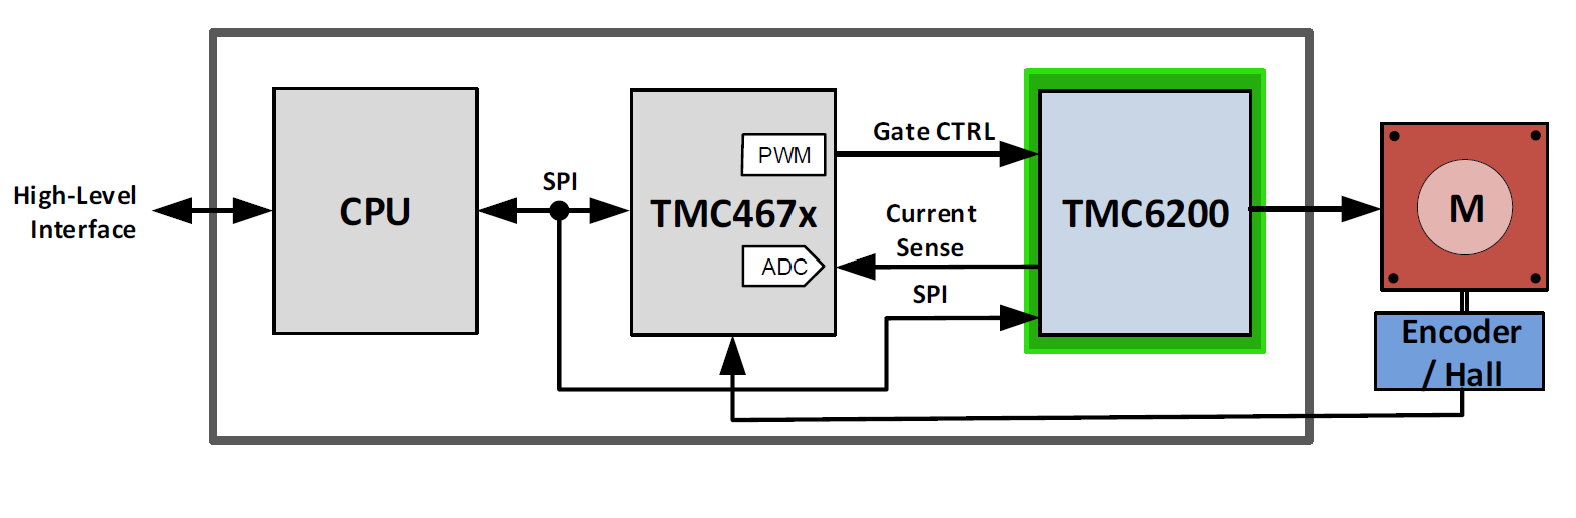
\includegraphics[width=0.8\textwidth]{graphics/Blockdiagramm_TMC4671_und_TMC6200}
	\caption{Blockschaltbild Konfiguration IC's mit BLDC und Encoder. \cite[S.1]{trinamicmotion_control_gmbh__co_kg_tmc6200_2019}}
	\label{fig:Blockdiagramm_TMC4671_und_TMC6200}
\end{figure}

%Es wurde darauf geachtet, dass der Aufbau des Prints dem Testaufbau entspricht. In Abbildung \ref{fig:Blockdiagramm_Motorengruppe} wird ein detaillierteres Blockschaltbild gezeigt, welches den Aufbau eher nach Funktionen beschreibt.

%\begin{figure}[H]
%	\centering
%	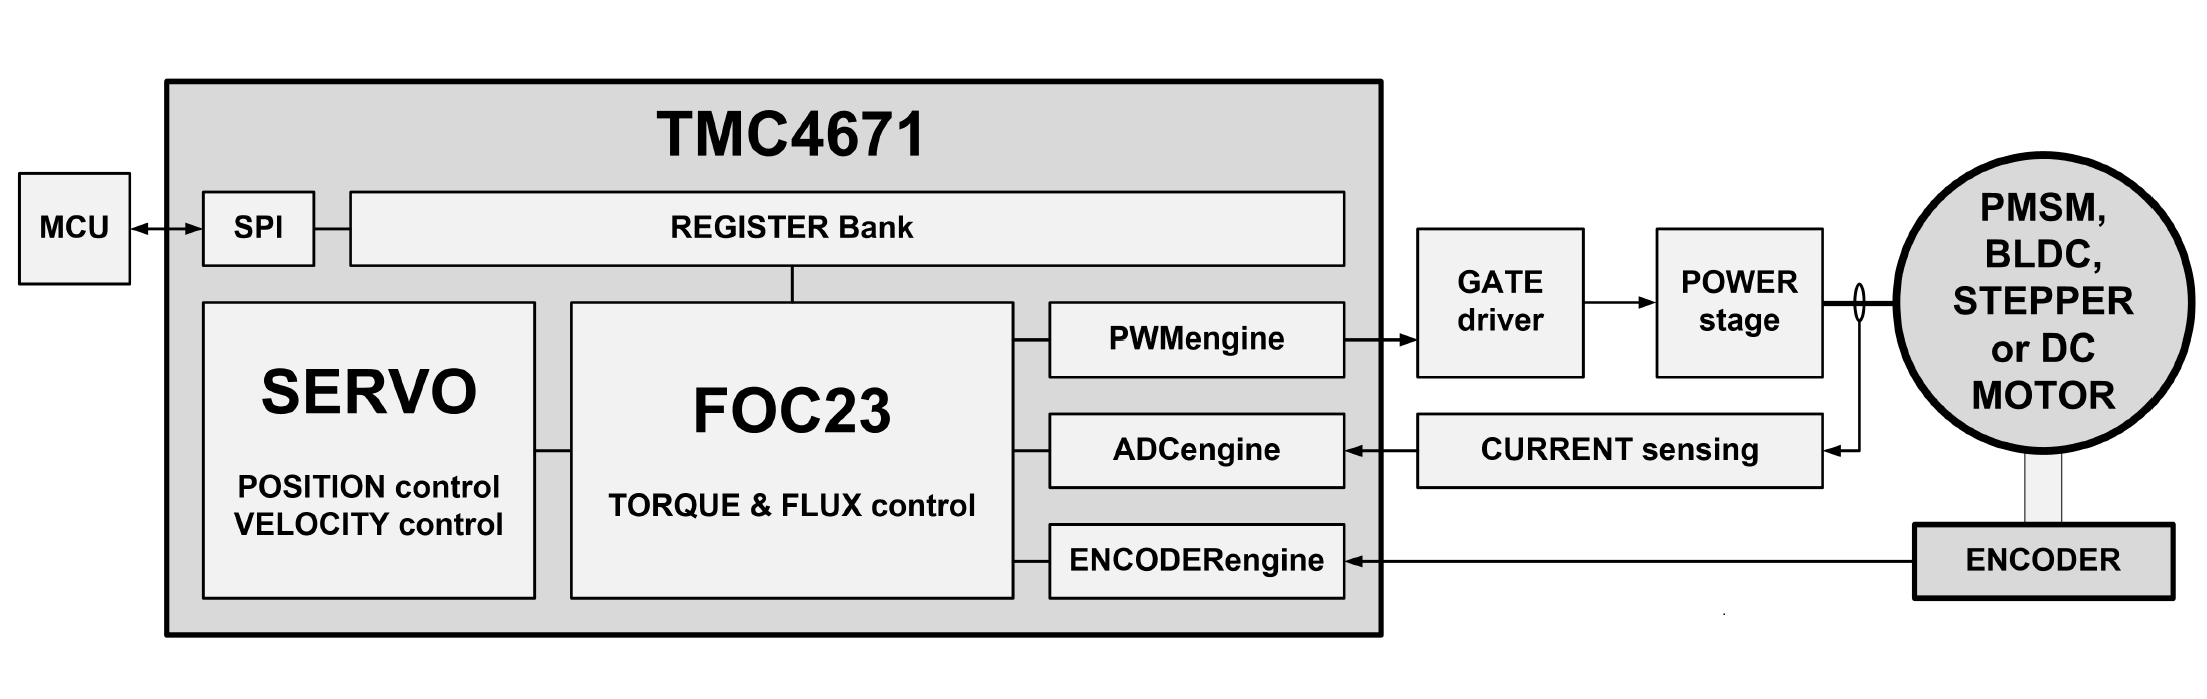
\includegraphics[width=0.8\textwidth]{graphics/Blockdiagramm_Motorengruppe}
%	\caption{Blockschaltbild Motorengruppe nach Funktionen. \cite[S.1]{trinamicmotion_control_gmbh__co_kg_tmc4671_2019}}
%	\label{fig:Blockdiagramm_Motorengruppe}
%\end{figure}

%\begin{table}[H]
%\center
%\begin{tabular}{|lll|l|}
%\hline
%\textbf{Kennzeichnung} & & \textbf{Bauteil} & \textbf{Funktion} \\
%\hline
%TMC4671 & = & Trinamic TMC4671 & FOC-Treiber \\
%GATE driver & = & Trinamic TMC6200 & Gate-Treiber \\
%POWER stage & = & Trnamic UPS 10A70V & H-Brücke \\
%Current sensing & = & UPS 10A70V ==> TMC6200 & Messung Phasenströme \\
%PMSM/BLDC & = & Sigmatec AKM22h & BLDC \\
%ENCODER & = & CUI devices ATS33 & ABN-Encoder \\
%\hline
%\end{tabular}
%\end{table}
%\newpage